\subsection{Overall accuracy of Simplified Ikeda method}
\label{se:overall_comparison}
An investigation of how well the implementation of the Simplified Ikeda method (see section \ref{se:simplified_ikeda}) agree with the corresponding result in the roll damping database has been carried out.

Figure \ref{fig:B_e_hat_ikeda} shows a comparison of the non dimensional equivalent linear damping $\hat{B_e}$
from model tests and the simplified method. Where predicted damping with Simplified Ikeda has been plotted against corresponding test in the roll damping database.  

\begin{figure}[H]
    \centering
    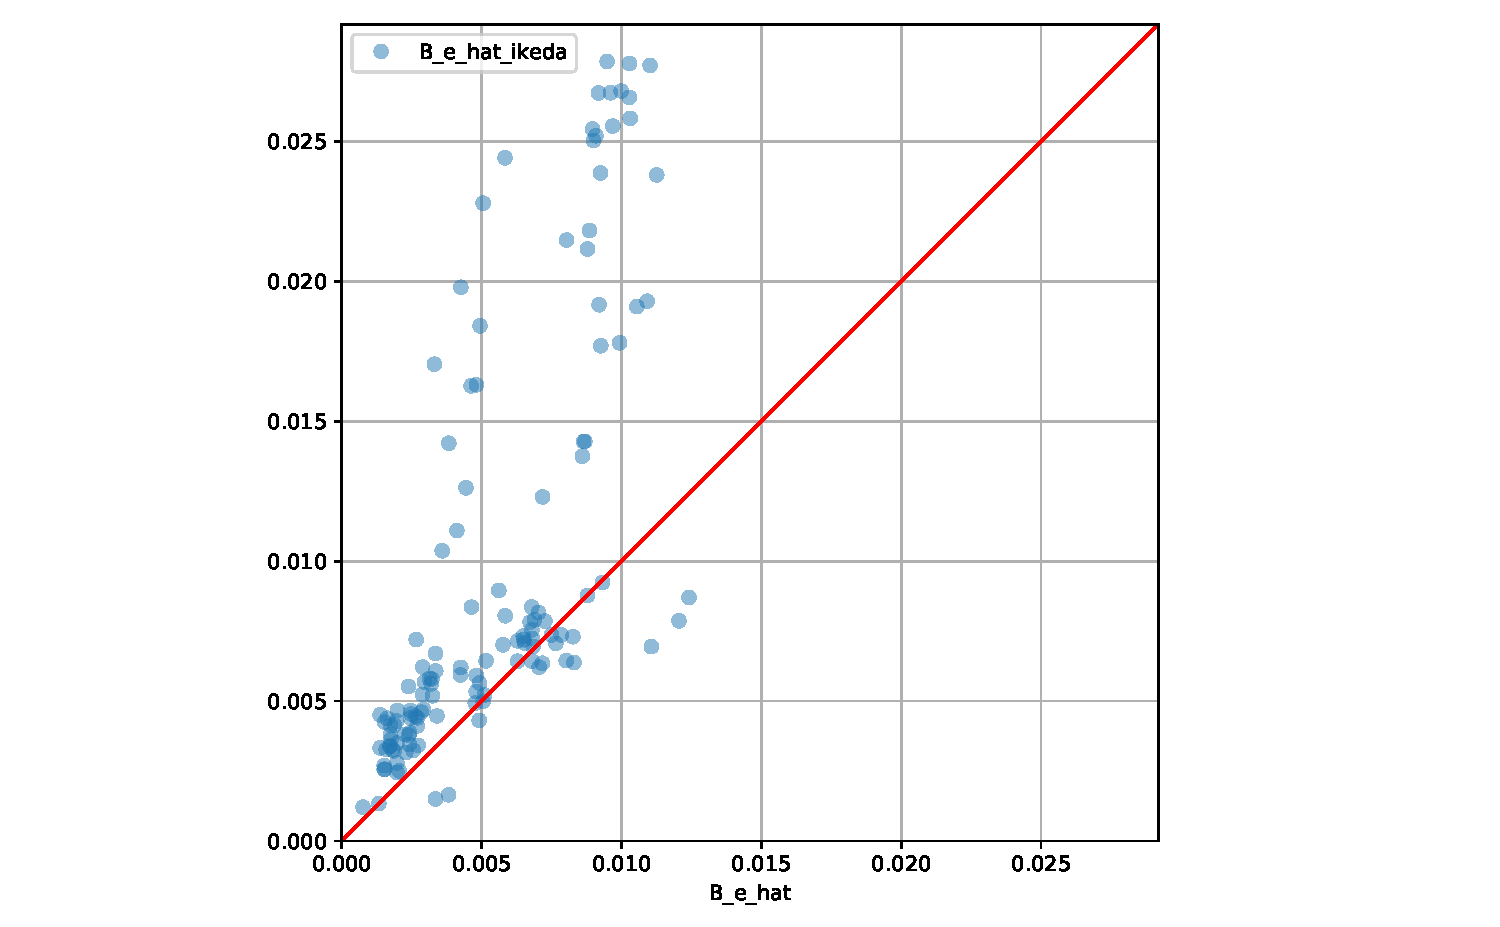
\includegraphics[width=\columnwidth]{figures/B_e_hat_ikeda.pdf}
    \caption{Nondimensional linearized damping from model tests and simplified Ikeda}
    \label{fig:B_e_hat_ikeda}
\end{figure}

The comparison show poor agreement. It was discovered that the prediction error was highly depending on the ship draught $T$ which is shown in figure  \ref{fig:B_e_hat_error}.
The figure shows that the error is much larger for $T/L_{pp}<0.034$.

\begin{figure}[H]
    \centering
    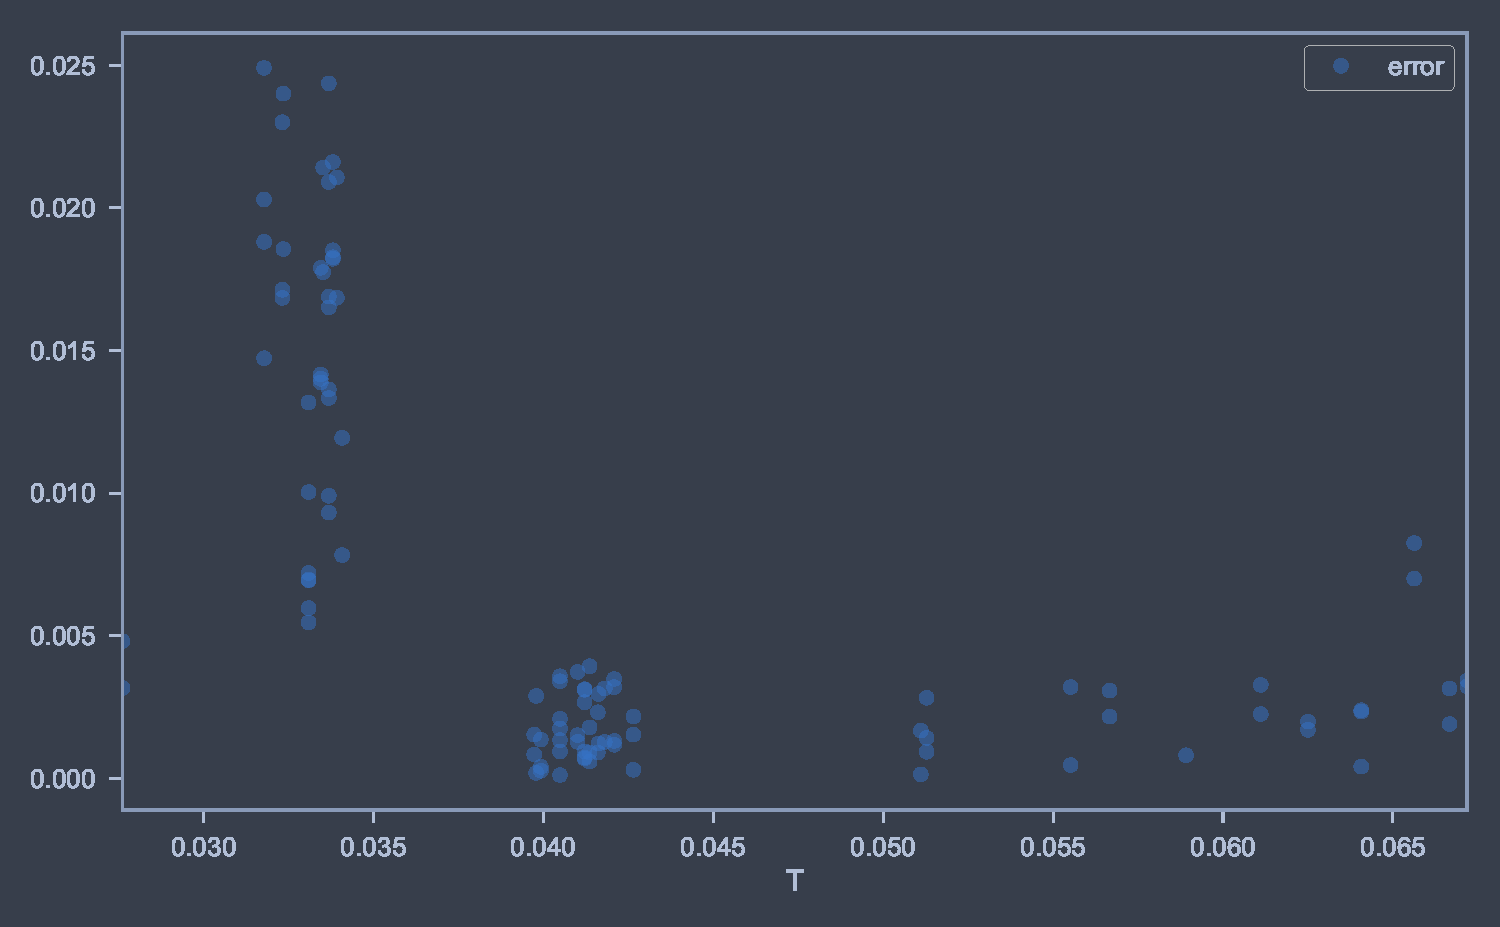
\includegraphics[width=\columnwidth]{figures/B_e_hat_error.pdf}
    \caption{Simplified Ikeda error versus draught}
    \label{fig:B_e_hat_error}
\end{figure}

Figure \ref{fig:B_e_hat_good} shows the comparison for only model tests with $T/L_{pp}>0.034$.
This confirms the small draft to beam ratio limit of this method as mentioned in \cite{kawahara_simple_2011}. The corresponding $R^2$ score is 0.38.

\begin{figure}[H]
    \centering
    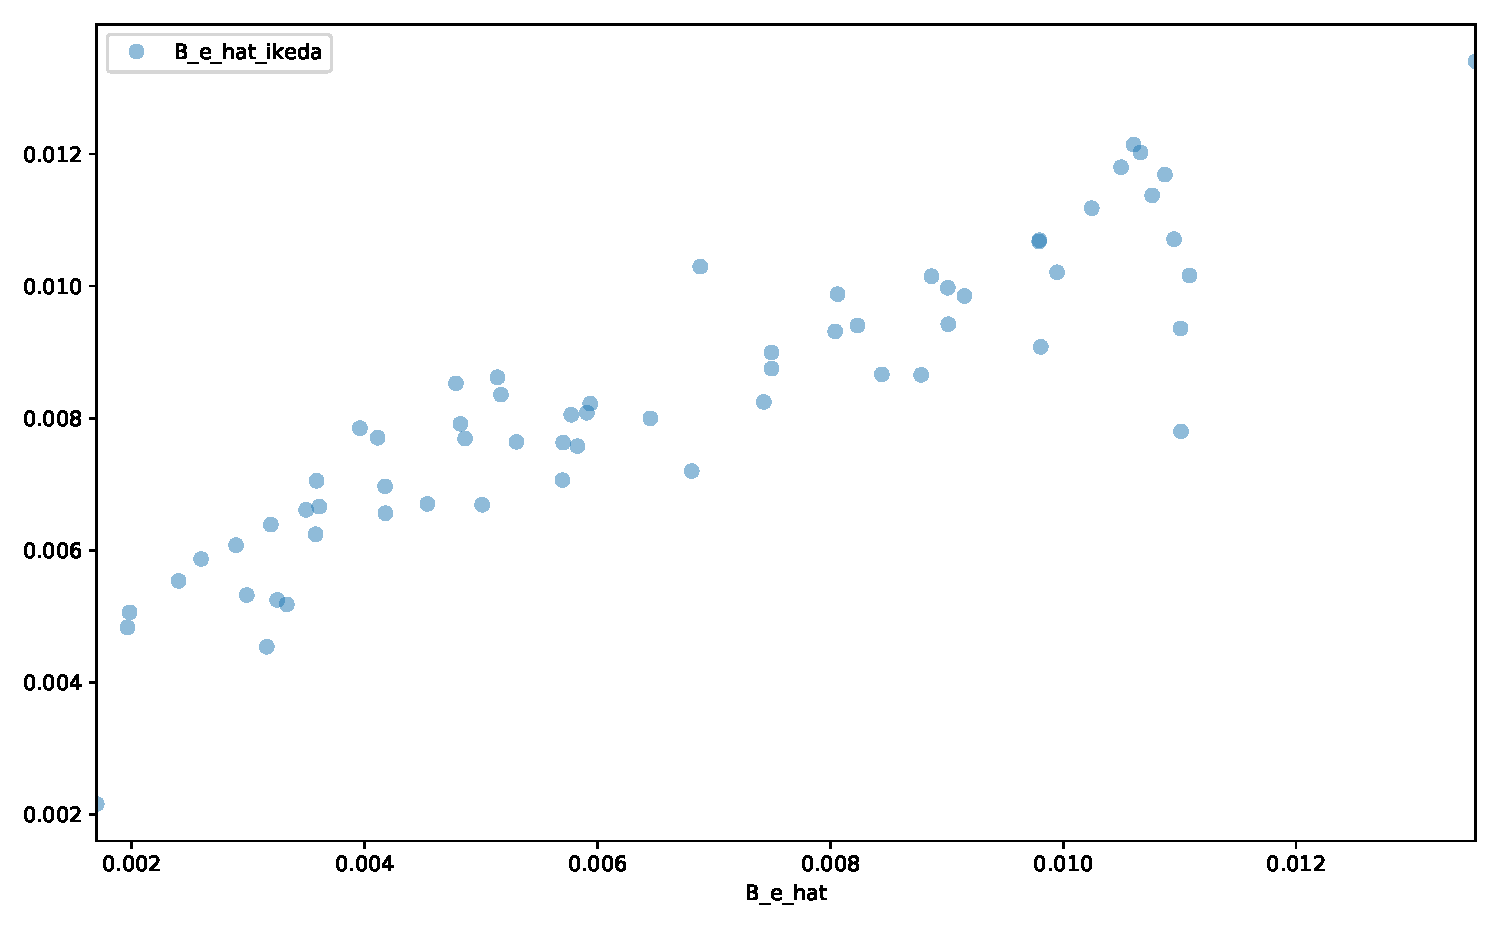
\includegraphics[width=\columnwidth]{figures/B_e_hat_good.pdf}
    \caption{Nondimensional linearized damping from model tests and simplified Ikeda $T/L_{pp}>0.034$}
    \label{fig:B_e_hat_good}
\end{figure}
